\documentclass{uofa-eng-assignment}

\usepackage{lipsum}
\usepackage{wrapfig}
\usepackage{caption}
\usepackage{subcaption}
\usepackage{float}
\usepackage[portuguese]{babel}
\usepackage[numbib]{tocbibind}
\usepackage{hyperref}
\usepackage{enumitem}

\newcommand*{\course}{Metodologias Experimentais em Informática}
\newcommand*{\assignment}{Assignment 3 -  Hypothesis testing}

\begin{document}
\begin{center}
    \textbf{\large \course}\\
    \assignment
\end{center}

\begin{center}
\begin{minipage}{0.3\textwidth}
\begin{center}Francisco Pires\\2019201225\\fjrp@student.dei.uc.pt\end{center}
\end{minipage}
\begin{minipage}{0.3\textwidth}
\begin{center}Gonçalo Pereira\\2008119715\\gnsp@student.dei.uc.pt\end{center}
\end{minipage}
\begin{minipage}{0.3\textwidth}
\begin{center}Tiago Delgado\\2021179681\\tiagodelgado@student.dei.uc.pt\end{center}
\end{minipage}
\end{center}

\section{Introdução}

Da análise exploratória da meta 1 foi possível concluir, sem margem para duvidas, que o algoritmo Dinic é de longe o mais performante dos três algoritmos estudados e que o EK é o menos. Posto isto, focamos o nosso estudo em cada algoritmo individualmente e excluímos a necessidade de validar estatisticamente diferenças entre os vários algoritmos.

Relembrando os modelos de regressão obtidos anteriormente: concluímos que o algoritmo Dinic seguia um modelo $O(|V|^2)$ e não o esperado $O(|A||V|^2)$; que o algoritmo MPM segue uma complexidade de $O(|A|^2)$ e não $O(|V|^3)$; e que o algoritmo EK segue a complexidade esperada de $O(|V||A|^2)$. De lembrar ainda que $|V|$ é o número de vértices do grafo, $|A|$ o número de arcos do grafo, e que $|A|$ foi estimado como $|A|=p\frac{n(n-1)}{2}$. $p$ e $n$ foram os nossos inputs para o gerador de grafos utilizado na análise experimental e correspondem à probabilidade de existência de arco entre dois vértices e ao número de vértices respetivamente.

Com estes resultados em mente, propusemos um estudo do impacto da variável $p$ nos vários algoritmos de modo a corroborar ou não os resultados anteriormente obtidos.

\section{Formulação de Hipóteses}
\label{sec:formulacao-hipoteses}

No nosso estudo pretendemos analisar e validar as seguintes hipóteses:

\begin{enumerate}[label=\emph{\Alph*} -]
\item O valor de p \textbf{não tem} impacto significativo no tempo de execução do algoritmo Dinic
\item O valor de p \textbf{tem} impacto significativo no tempo de execução do algoritmo MPM
\item O valor de p \textbf{tem} impacto significativo no tempo de execução do algoritmo EK
\end{enumerate}

No caso da hipótese \emph{A}, $p$ não ter impacto significativo no tempo de execução irá permitir provar que a complexidade temporal do algoritmo não depende do número de arcos $|A|$ --- estimado como $|A|=p\frac{n(n-1)}{2}$. Para a hipótese \emph{B}, $p$ ter impacto significativo no tempo de execução irá permitir provar que a complexidade temporal não depende apenas do número de vértices $|V|$. Finalmente a hipótese \emph{C} servirá simplesmente como teste de sanidade pois para o algoritmo EK não se observou qualquer divergência com o comportamento esperado.

\section{Design da experiência}

De modo a validar as 3 hipóteses anteriormente definidas, fizemos 3 testes estatísticos usando o modelo estatístico 2-way ANOVA. O teste estatístico “Two-Way” ANOVA é utilizado quando se pretende estudar o efeito de duas variáveis independentes e como estas interagem entre si e afetam o valor final da variável dependente. No nosso caso pretendemos estudar $n$, $p$ e eventuais interações entre ambas. Para cada algoritmo pretendemos testar as hipóteses:

\begin{itemize}
\item $H_0^1$: Não existem diferenças entre as médias do fator $n$
\item $H_1^1$: As médias do fator $n$ não são iguais
\end{itemize}
\begin{itemize}
\item $H_0^2$: Não existem diferenças entre as médias do fator $p$
\item $H_1^2$: As médias do fator $p$ não são iguais
\end{itemize}
\begin{itemize}
\item $H_0^3$: Não existem diferenças entre as médias da interação dos fatores $n$ e $p$
\item $H_1^3$: As médias da interação dos fatores $n$ e $p$ não são iguais
\end{itemize}

De modo a utilizar os resultados obtidos nos testes Two-way ANOVA, será necessário verificar ainda os pressupostos: normalidade dos resíduos e a "homoskedasticity" (homogeneidade de variâncias). É ainda necessário garantir a independência das observações, mas tal foi garantido no desenho experimental ao utilizar diferences valores de $s$ (seed).

Para validar a normalidade dos resíduos recorremos ao teste Shapiro-Wilk. A hipótese nula é que os resíduos seguem uma distribuição normal, enquanto a hipótese alternativa é que os resíduos não seguem uma distribuição normal.
Para validar a homoskedasticity recorremos ao teste de Levene e à visualização dos resíduos usando um "Residuals-vs-fitted" plot. A hipótese nula é que as variâncias dos dois grupos são iguais, enquanto a hipótese alternativa é que as variâncias não são iguais.

Nos casos em os pressupostos sejam verificados iremos proceder a uma analise Post-Hoc dos factores usando um teste TukeyHSD. Caso não sejam verificados será necessário usar uma alternativa não paramétrica.

Existem poucas alternativas não paramétricas à Two-Way ANOVA, e portanto iremos efectuar um teste de aleatorização de permutações sem restrições com o intuito de observar se existem diferenças entre as médias para um nível de significância de 5\%. Um teste de aleatorização é um procedimento em que se comparam valores de uma estatística observada nos dados com os valores desta estatística após a aleatorização das observações. A principal vantagem da utilização deste teste é que pode ser utilizado para pequenas amostras, aleatórias ou não, e como se trata de um teste não-paramétrico, prescinde da distribuição da população da qual a amostra foi extraída.

\section{Resultados Dinic}

\subsection{Visualização dos dados e interações}
No gráfico demonstrado na figura \ref{fig:boxplot-dinic-p} é possível afirmar que, para o algoritmo Dinic, a probabilidade aparenta ter impacto no tempo de execução. Embora para $p = 0.1$ e $p = 0.9$ as respostas sejam relativamente iguais, para $p = 0.5$ podemos observar um comportamento diferente onde para maiores valores de $n$ se observa uma maior variância nos tempos de execução.
Como podemos observar na figura \ref{fig:boxplot-dinic-n}, um aumento do número de vértices tem um impacto direto na variável de resposta (tempo).

\begin{figure}[h]
    \begin{minipage}{0.45\textwidth}
        \centering
        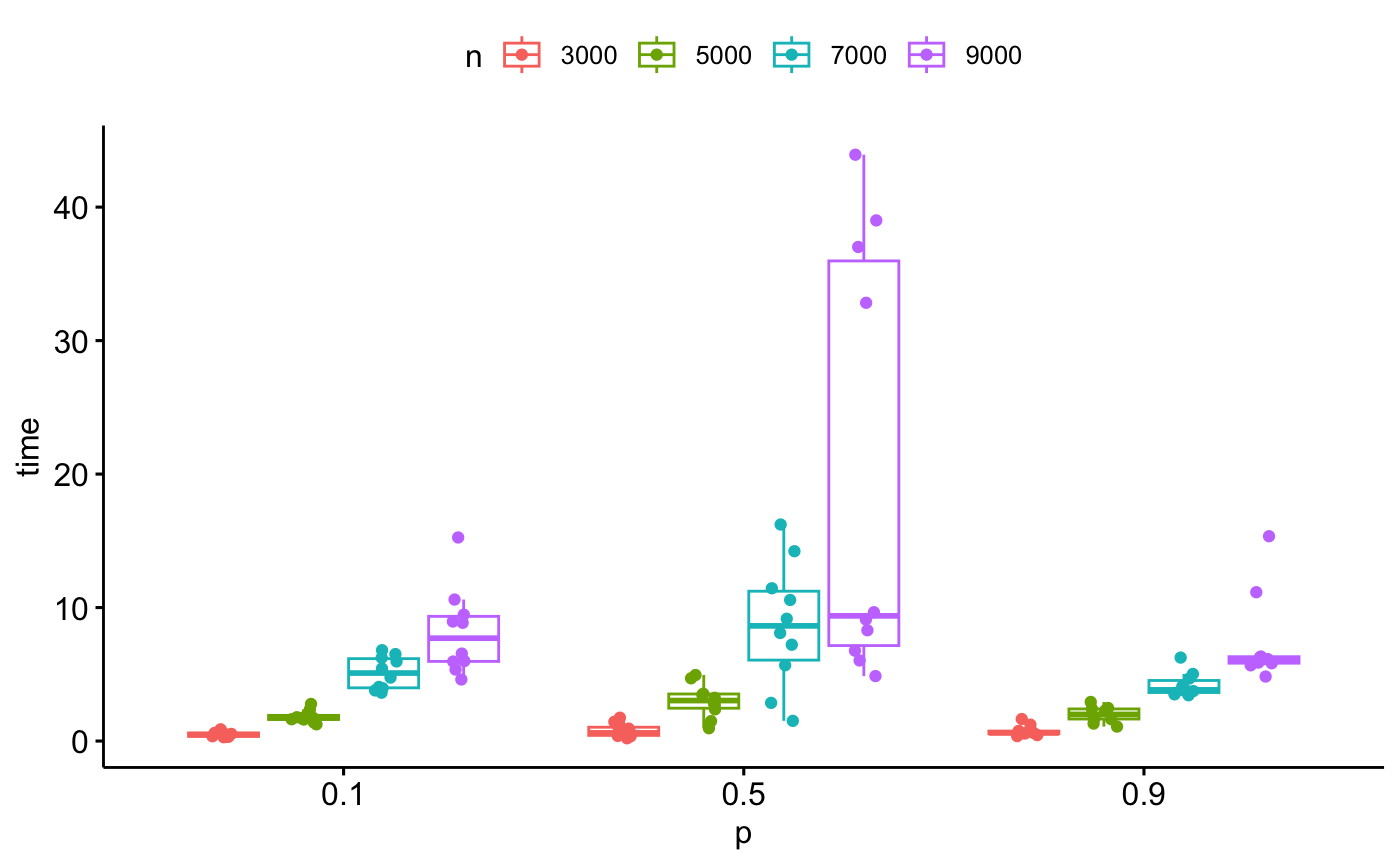
\includegraphics[width=.7\linewidth]{plot.png}
        \caption{Dinic boxplot para $p$}
        \label{fig:boxplot-dinic-p}
    \end{minipage}
    \hfill
    \begin{minipage}{0.45\textwidth}
        \centering
        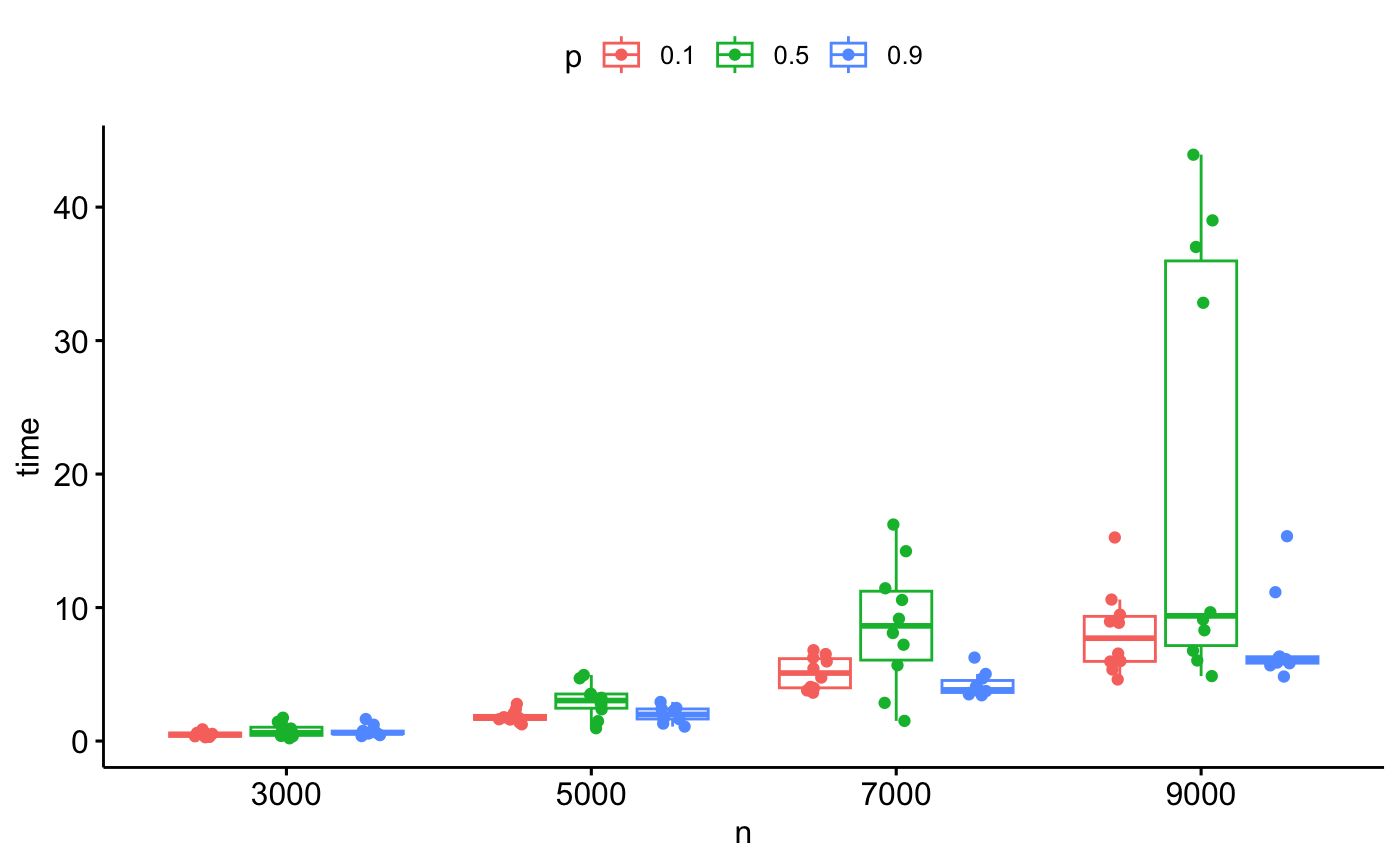
\includegraphics[width=.7\linewidth]{plot2.png}
        \caption{Dinic boxplot para $n$}
        \label{fig:boxplot-dinic-n}
    \end{minipage}
\end{figure}

Olhando para os interaction plots das figuras \ref{fig:intplot-dinic-n} e \ref{fig:intplot-dinic-p}, podemos confirmar as conclusões retiradas anteriormente. Com esta visualização é particularmente fácil de observar uma interação entre as variáveis $n$ e $p$. Para $n = 9000$ é possível ver nas duas figuras o impacto de $p = 0.5$ face aos restantes valores --- isto é, as linhas não são paralelas.

\begin{figure}[h]
    \begin{minipage}{0.45\textwidth}
        \centering
        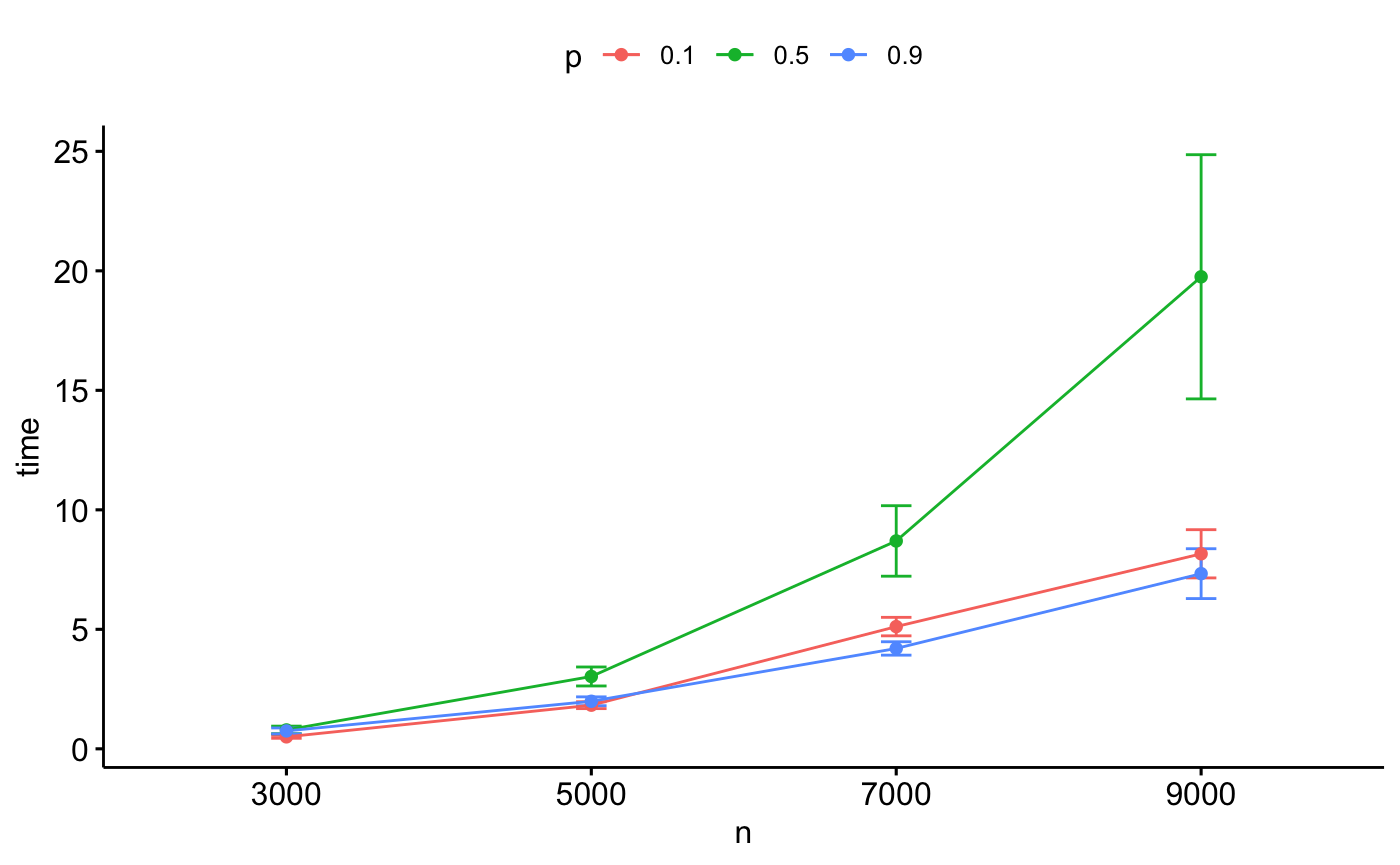
\includegraphics[width=1\linewidth]{intplot1.png}
        \caption{Dinic Interaction Plot para $n$}
        \label{fig:intplot-dinic-n}
    \end{minipage}\hfill
    \begin{minipage}{0.45\textwidth}
        \centering
        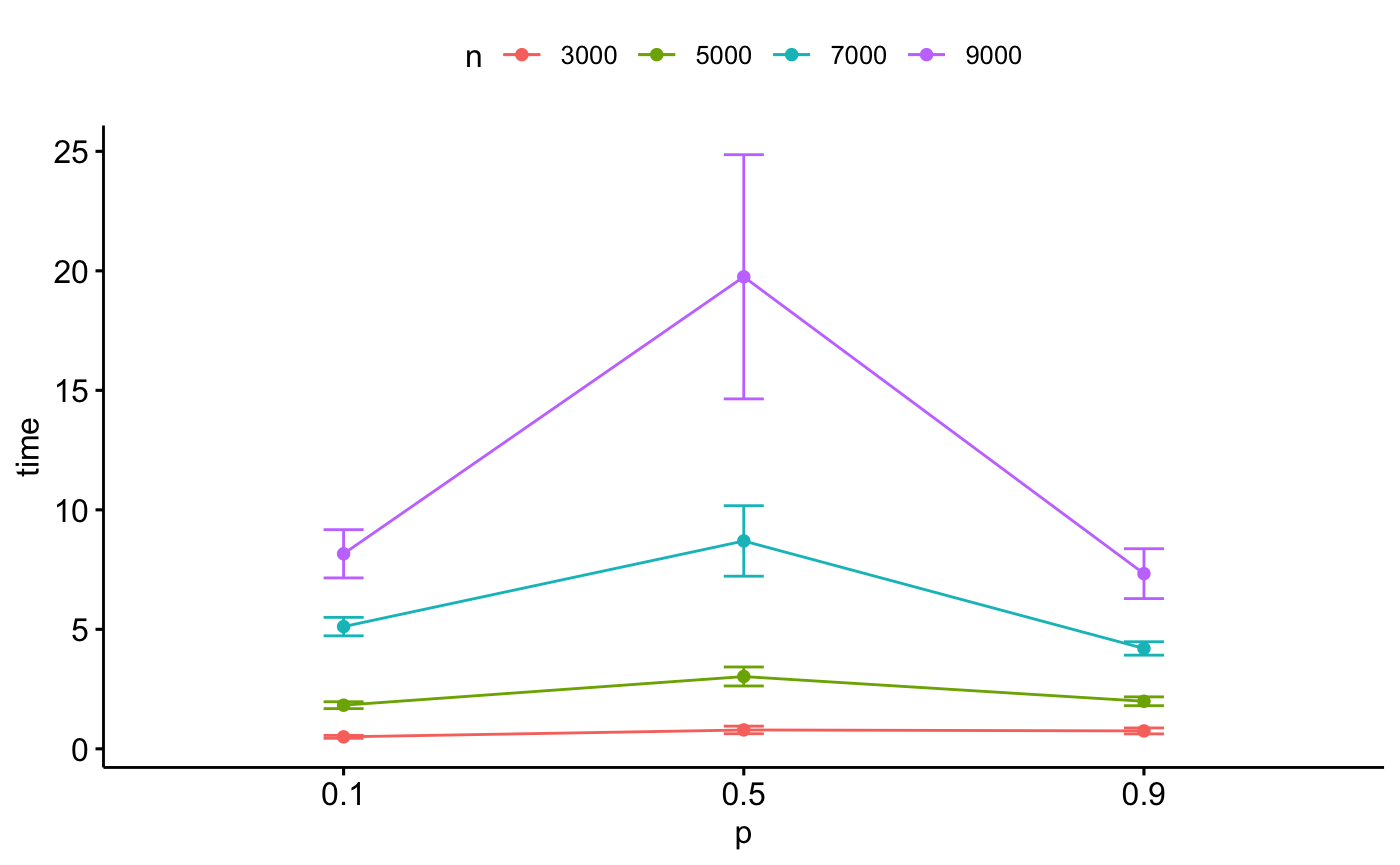
\includegraphics[width=1\linewidth]{intplot2.png}
        \caption{Dinic Interaction Plot para $p$}
        \label{fig:intplot-dinic-p}
    \end{minipage}
\end{figure}

\subsection{Teste Two-Way ANOVA}

Em seguida é mostrada a tabela \ref{fig:anova-dinic} obtida utilizando a função \emph{aov} do R para analisar os resultados obtidos e tomar uma decisão de rejeitar ou não rejeitar as hipóteses.

\begin{figure}[h]
    \centering
    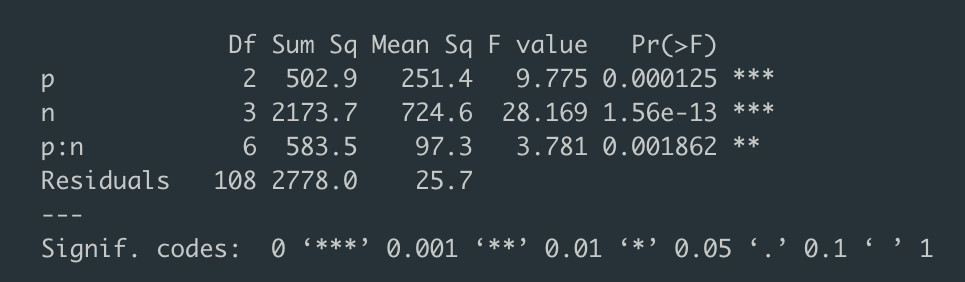
\includegraphics[width=0.7\textwidth]{anova-dinic.png}
    \caption{Tabela ANOVA Dinic}
    \label{fig:anova-dinic}
\end{figure}

\subsection{Validação pressupostos ANOVA}

Na figura \ref{fig:resplot-dinic} podemos ver um ligeiro afastamento da linha a vermelho sobre o tracejado. Na figura \ref{fig:pressupostos-dinic} podemos observar que tanto para o teste de Levene como para o teste de Shapiro-Wilk rejeitamos ambas as hipóteses nulas dos testes.

\begin{figure}[h]
    \begin{minipage}{0.45\textwidth}
        \centering
        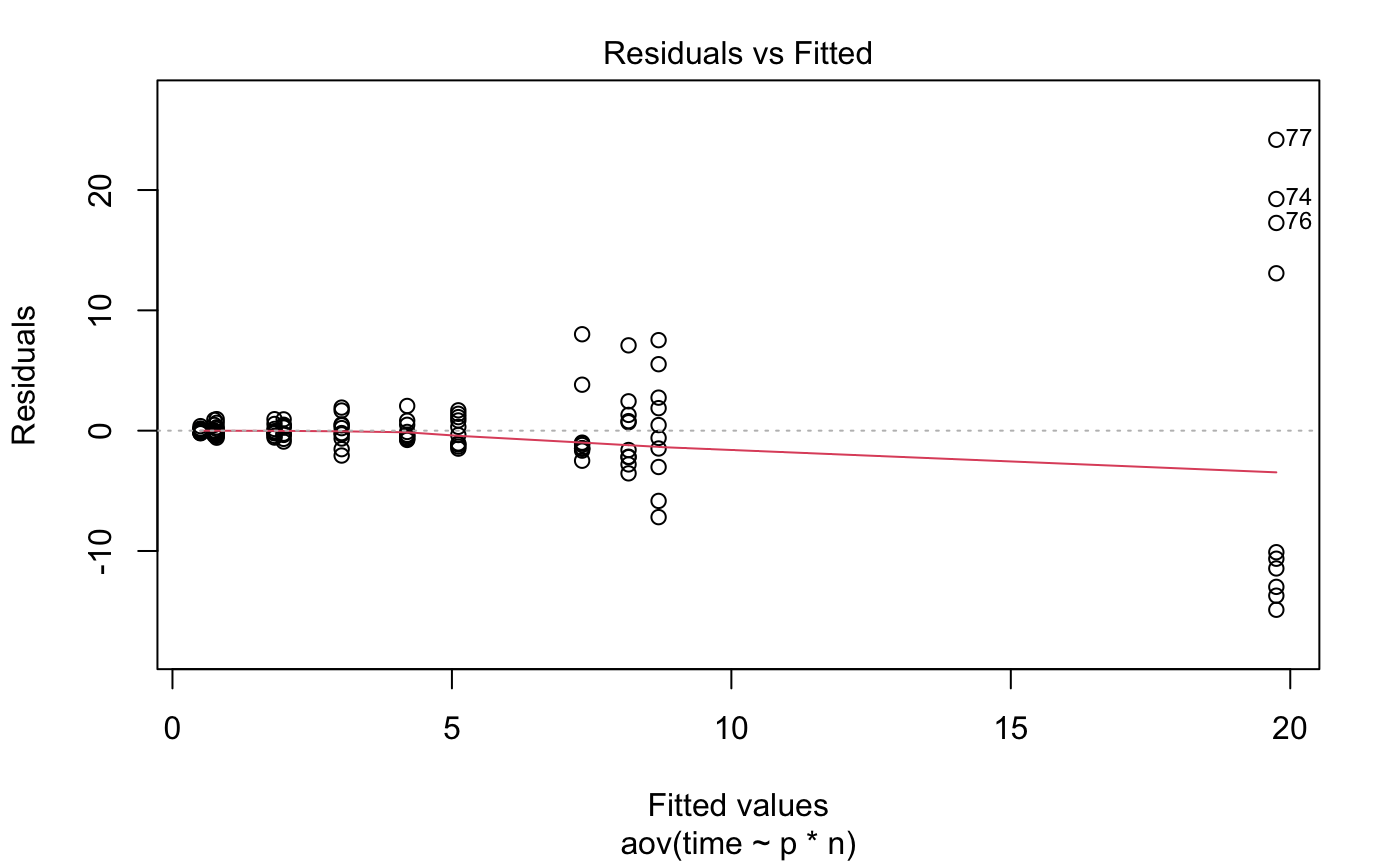
\includegraphics[width=1\textwidth]{resplot-dinic.png}
        \caption{Dinic Residuals vs Fitted plot}
        \label{fig:resplot-dinic}
    \end{minipage}
    \hfill
    \begin{minipage}{0.45\textwidth}
        \centering
        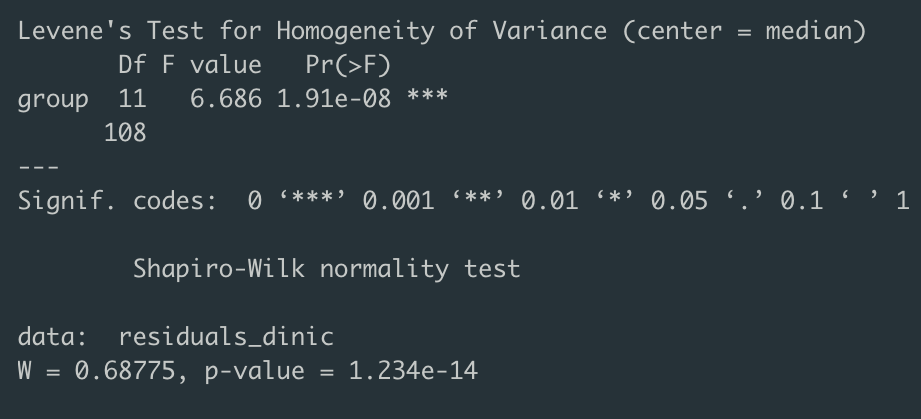
\includegraphics[width=1\textwidth]{pressupostos_dinic.png}
        \caption{Pressupostos ANOVA}
        \label{fig:pressupostos-dinic}
    \end{minipage}
\end{figure}

\subsection{Alternativa não paramétrica para Two-Way ANOVA}

Após verificar os pressupostos ANOVA, foi possível concluir que os pressupostos de normalidade e a homogeneidade das variações não foram validados. Dado isto foi utilizada a alternativa não paramétrica e os resultados podem ser observados na figura \ref{fig:randtest-dinic}

\begin{figure}[h]
    \centering
    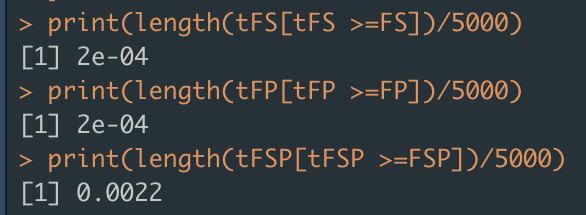
\includegraphics[width=0.5\linewidth]{rand_test_dinic.png}
    \caption{Randomization test Dinic}
    \label{fig:randtest-dinic}
\end{figure}


\section{Resultados MPM}

\subsection{Visualização dos dados e interações}

Com o gráfico demonstrado na figura \ref{fig:boxplot-mpm-p} é possível afirmar que para o algoritmo MPM quanto maior for a probabilidade maior irá ser o tempo de execução do código, onde existem alguns outliers sobretudo na probabilidade 0.9.
Como podemos observar na Figura \ref{fig:boxplot-mpm-n}, quanto maior for o número de vértices para o algoritmo MPM, maior irá ser o tempo de execução do algoritmo, o que implica que o número de vértices tem implicação direta no tempo.

\begin{figure}[h]
    \begin{minipage}{0.45\textwidth}
        \centering
        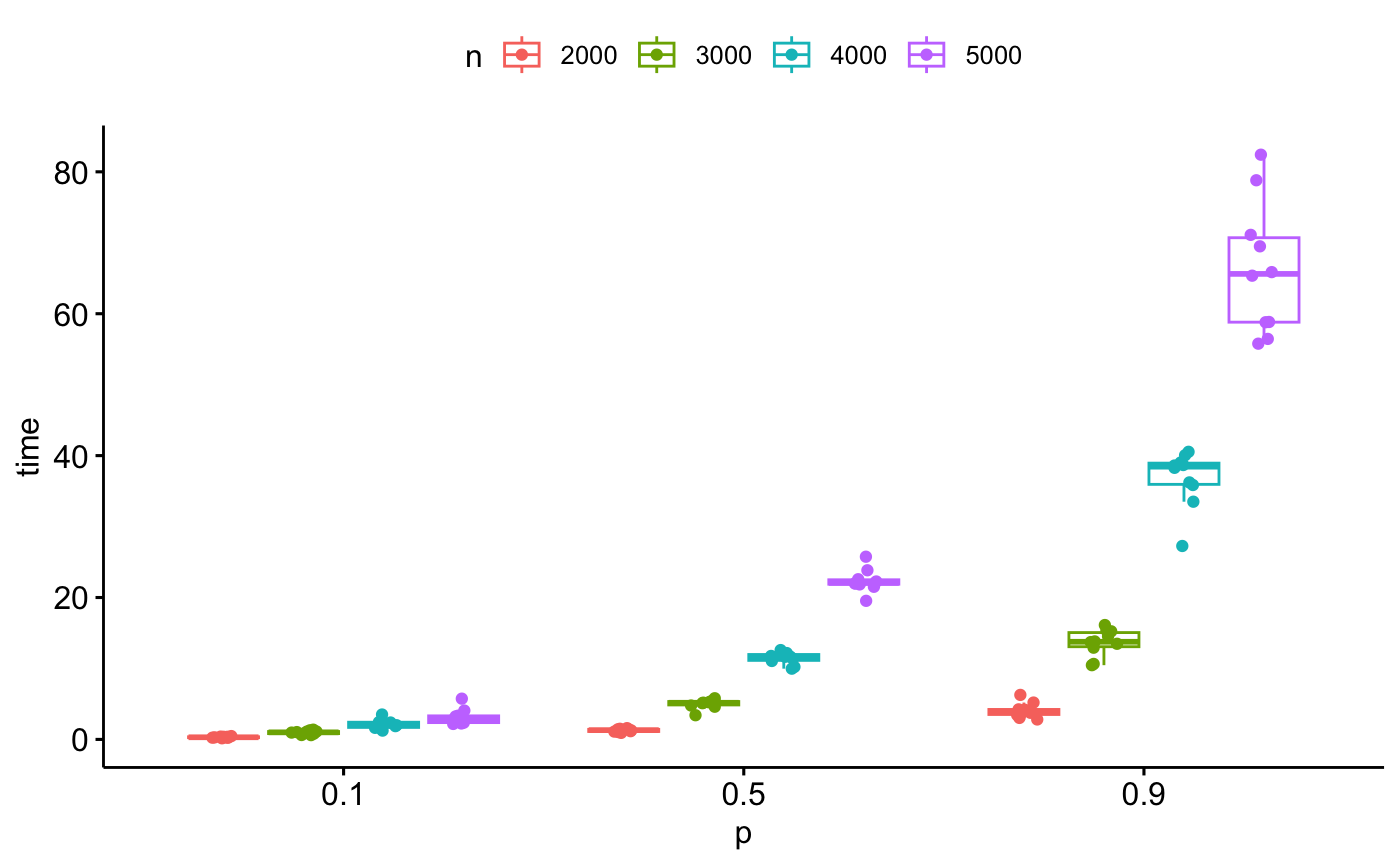
\includegraphics[width=.7\linewidth]{mpm_plot2.png}
        \caption{MPM boxplot para $p$}
        \label{fig:boxplot-mpm-p}
    \end{minipage}
    \hfill
    \begin{minipage}{0.45\textwidth}
        \centering
        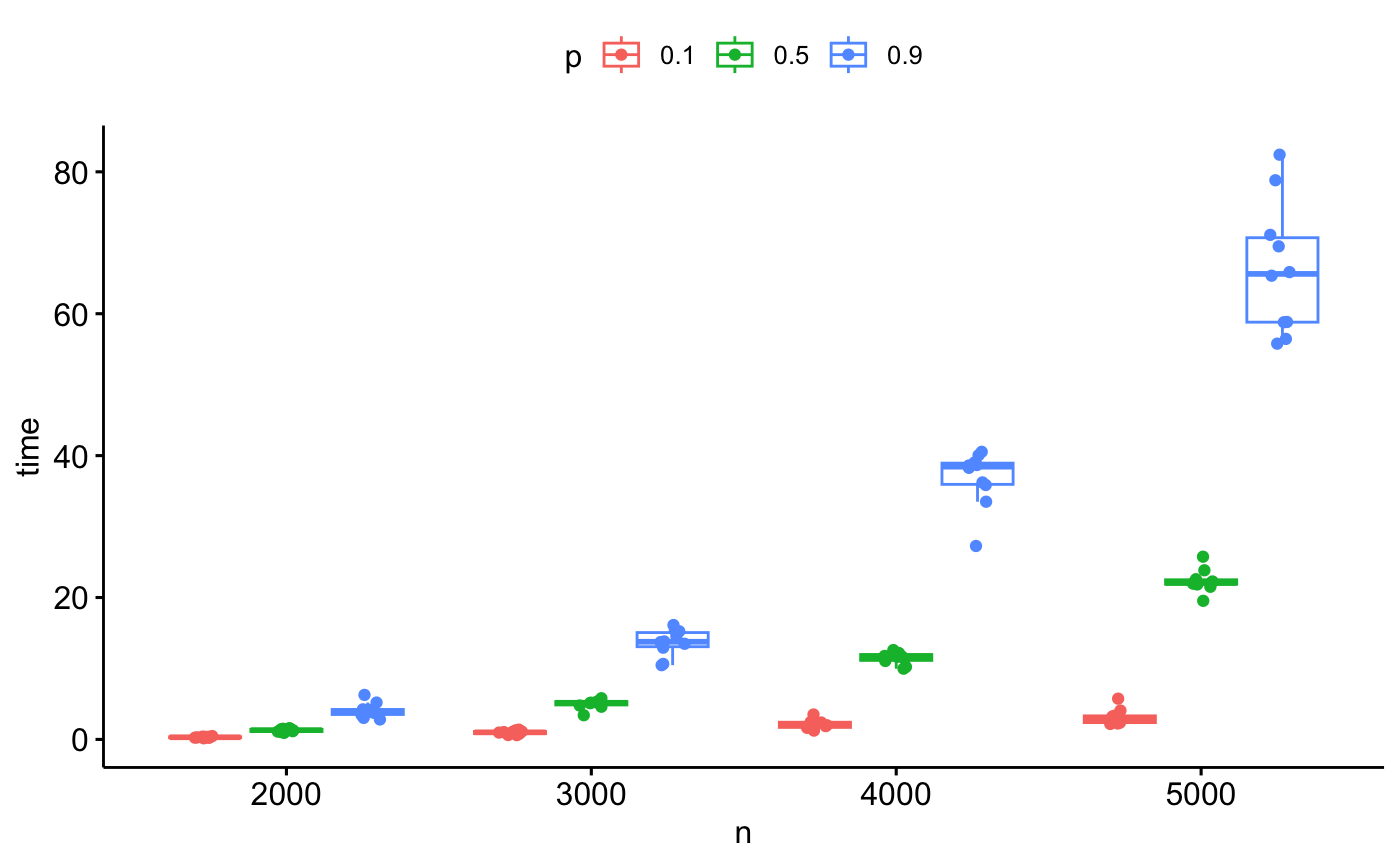
\includegraphics[width=.7\linewidth]{mpm_plot1.png}
        \caption{MPM boxplot para $n$}
        \label{fig:boxplot-mpm-n}
    \end{minipage}
\end{figure}

Como podemos observar pelos interaction plots das figuras \ref{fig:intplot-mpm-n} e \ref{fig:intplot-mpm-p}, podemos observar que existe uma interação clara entre as diferentes probabilidades e número de vértices.

\begin{figure}[h]
    \begin{minipage}{0.45\textwidth}
        \centering
        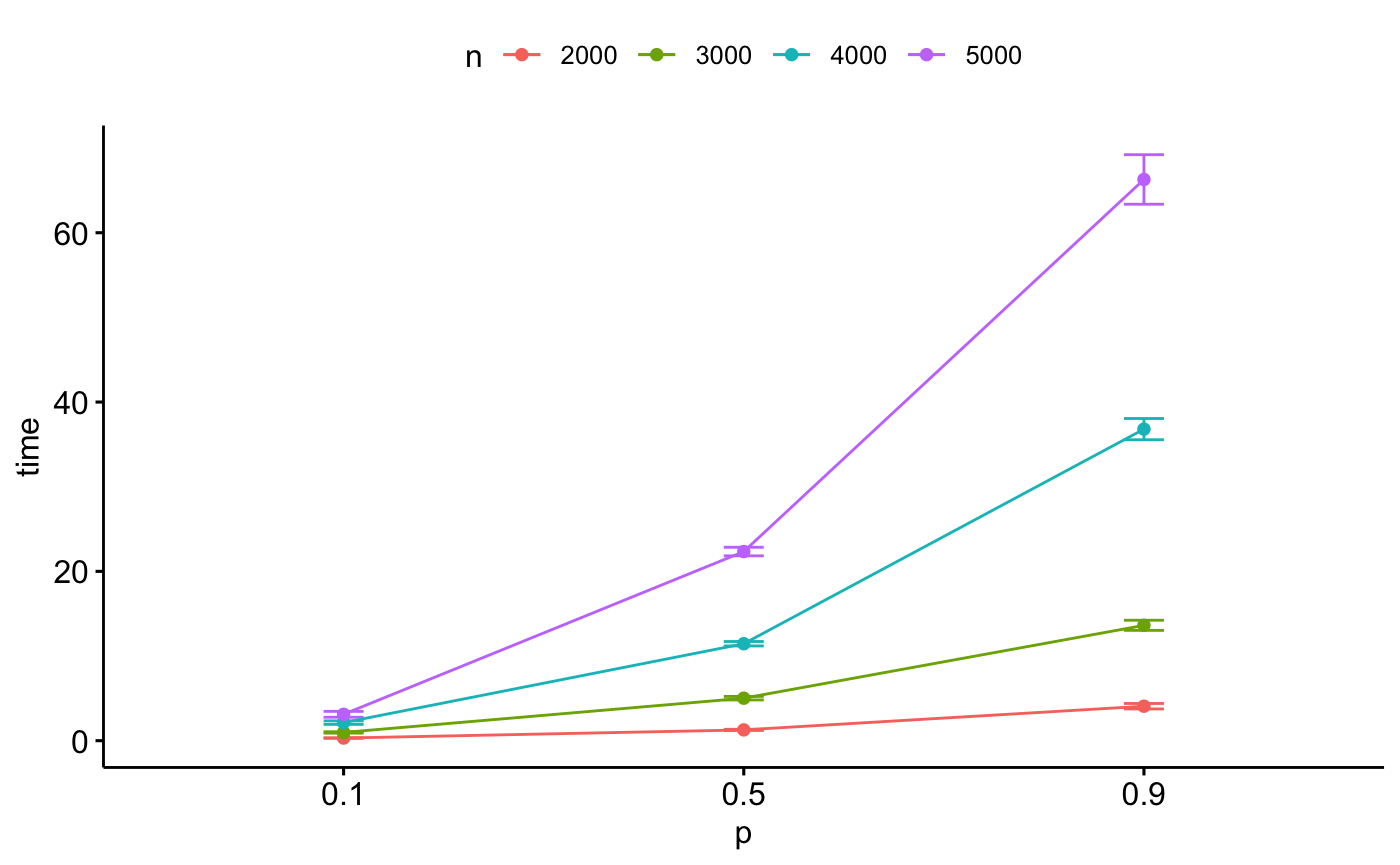
\includegraphics[width=1\linewidth]{mpm_intplot1.png}
        \caption{Mpm boxplot para $p$}
        \label{fig:intplot-mpm-n}
    \end{minipage}\hfill
    \begin{minipage}{0.45\textwidth}
        \centering
        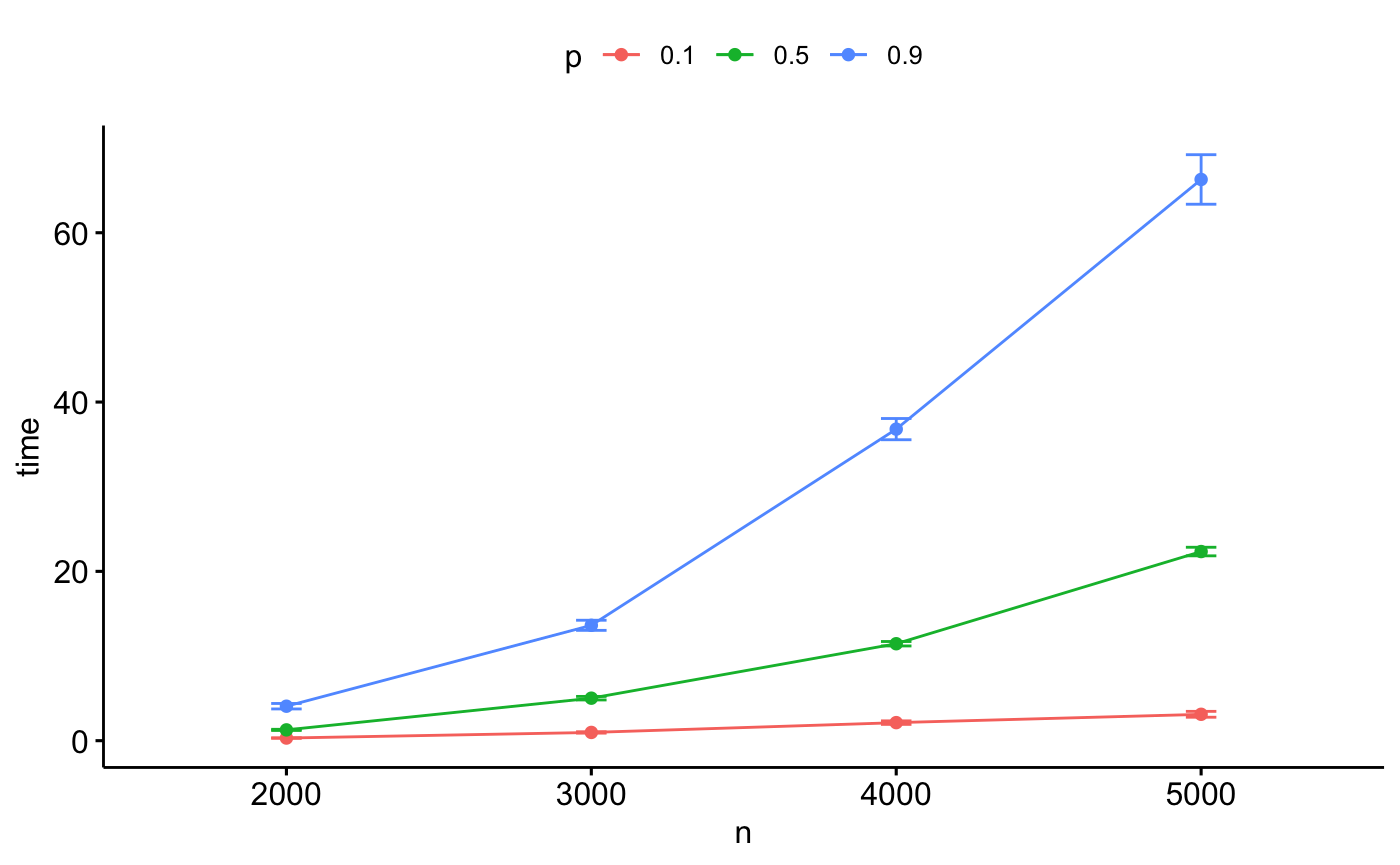
\includegraphics[width=1\linewidth]{mpm_intplot2.png}
        \caption{Mpm boxplot para $n$}
        \label{fig:intplot-mpm-p}
    \end{minipage}
\end{figure}

\subsection{Teste Two-Way ANOVA}

Em seguida é mostrada a tabela \ref{fig:anova-mpm} obtida utilizando a função \emph{aov} do R para analisar os resultados obtidos e tomar uma decisão de rejeitar ou não rejeitar as hipóteses.

\begin{figure}[h]
    \centering
    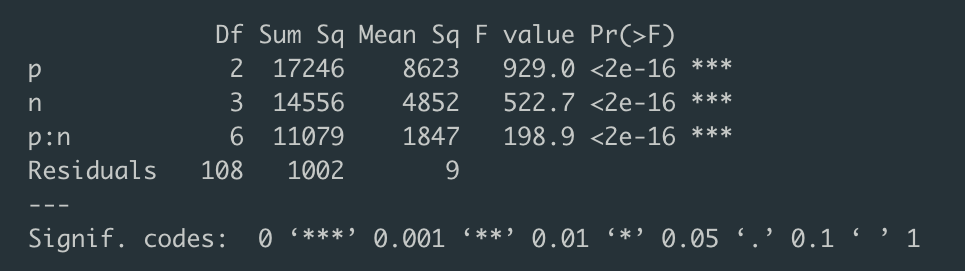
\includegraphics[width=0.7\textwidth]{mpm-anova.png}
    \caption{Tabela ANOVA MPM}
    \label{fig:anova-mpm}
\end{figure}

\subsection{Validação pressupostos ANOVA}

Na figura \ref{fig:resplot-mpm} podemos ver um ligeiro afastamento da linha a vermelho sobre o tracejado. Na figura \ref{fig:pressupostos-mpm} podemos observar que tanto para o teste de Levene como para o teste de Shapiro-Wilk rejeitamos ambas as hipóteses nulas dos testes. 

\begin{figure}[h]
    \begin{minipage}{0.45\textwidth}
        \centering
        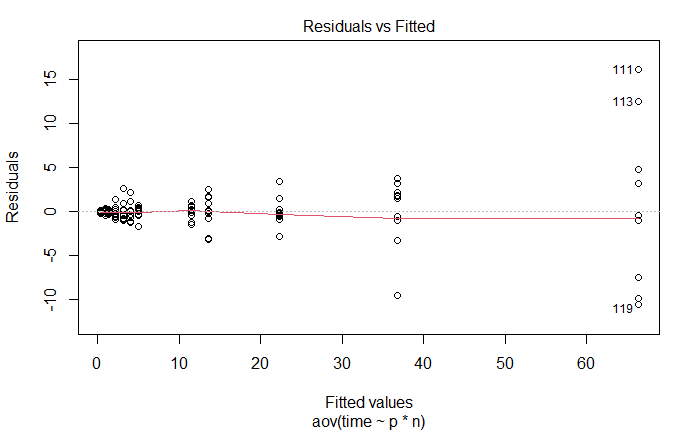
\includegraphics[width=1\textwidth]{res_plot_mpm.png}
        \caption{Mpm Residuals vs Fitted plot}
        \label{fig:resplot-mpm}
    \end{minipage}
    \hfill
    \begin{minipage}{0.45\textwidth}
        \centering
        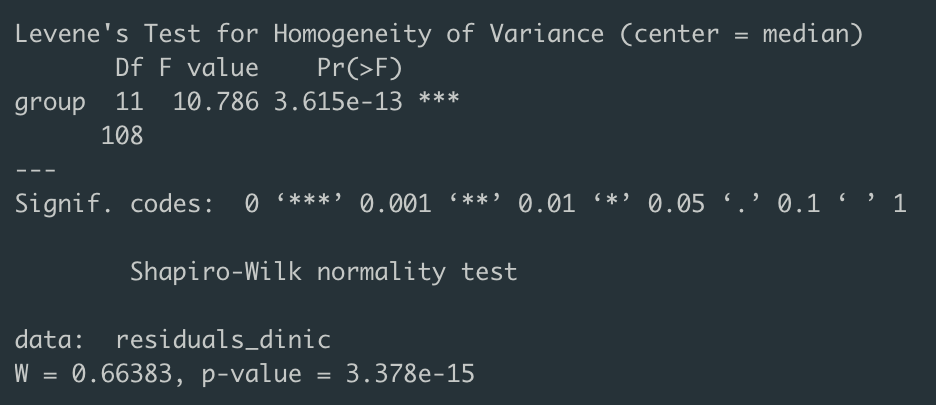
\includegraphics[width=1\textwidth]{pressupostos_mpm.png}
        \caption{Pressupostos ANOVA}
        \label{fig:pressupostos-mpm}
    \end{minipage}
\end{figure}

\subsection{Alternativa não paramétrica para Two-Way ANOVA}

Após verificar os pressupostos ANOVA, foi possível concluir que os pressupostos de normalidade e a homogeneidade das variações não foram validados. Dado isto foi utilizada a alternativa não paramétrica e os resultados podem ser observados na figura \ref{fig:randtest-mpm}

\begin{figure}[h]
    \centering
    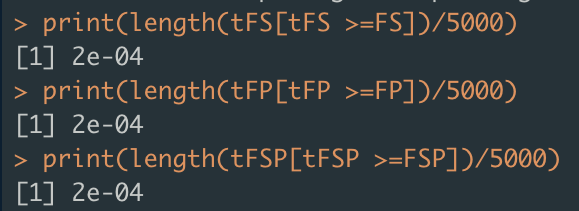
\includegraphics[width=0.5\linewidth]{randomization_mpm.png}
    \caption{Randomization test MPM}
    \label{fig:randtest-mpm}
\end{figure}


\section{Resultados EK}

\subsection{Visualização dos dados e interações}

O algoritmo EK aparenta ter um comportamento e conclusões semelhantes ao MPM como se pode ver pelas figuras \ref{fig:boxplot-ek-n}, \ref{fig:boxplot-ek-p}, \ref{fig:intplot-ek-n} e \ref{fig:intplot-ek-p}. Tanto $n$ como $p$ impactam a variável de resposta como parece haver interacções.

\begin{figure}[h]
    \begin{minipage}{0.45\textwidth}
        \centering
        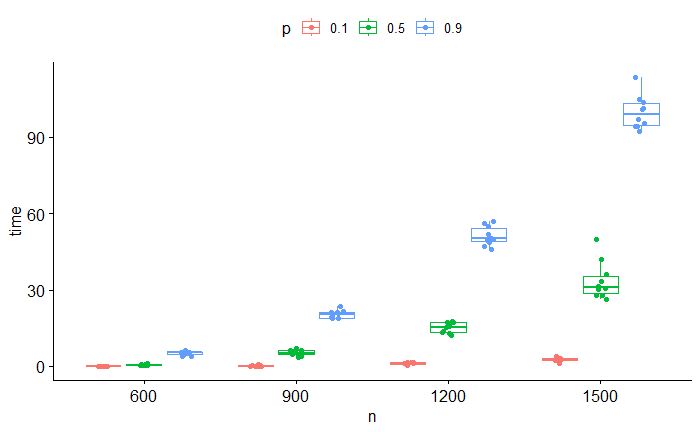
\includegraphics[width=.7\textwidth]{ek_plot1.png}
        \caption{EK boxplot para $n$}
        \label{fig:boxplot-ek-n}
    \end{minipage}
    \hfill
    \begin{minipage}{0.45\textwidth}
        \centering
        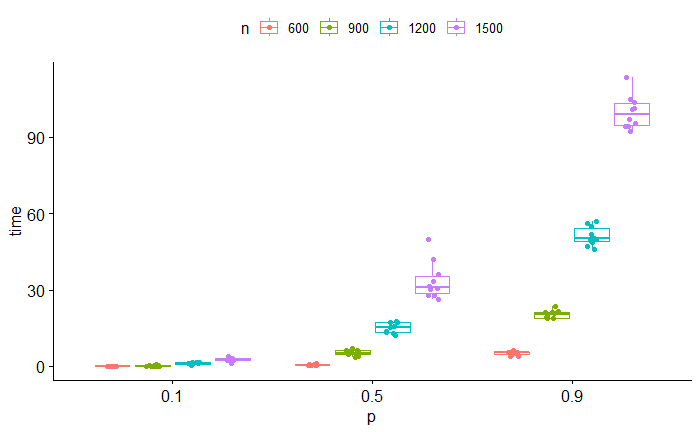
\includegraphics[width=.7\textwidth]{ek_plot2.png}
        \caption{EK boxplot para $p$}
        \label{fig:boxplot-ek-p}
    \end{minipage}
\end{figure}

\begin{figure}[h]
    \begin{minipage}{0.45\textwidth}
        \centering
        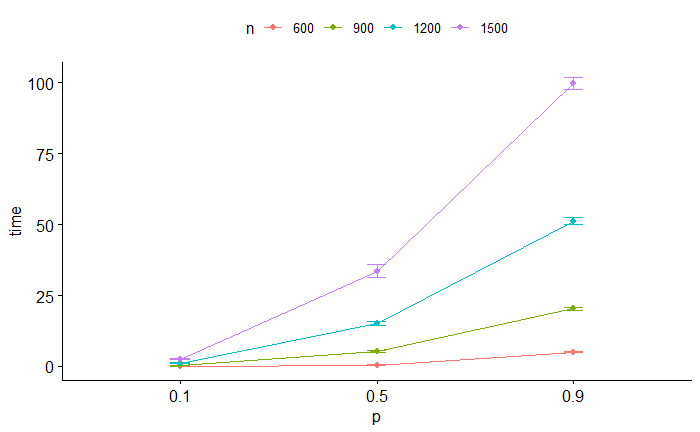
\includegraphics[width=1\textwidth]{ek_intplot1.png}
        \caption{EK boxplot para $n$}
        \label{fig:intplot-ek-n}
    \end{minipage}\hfill
    \begin{minipage}{0.45\textwidth}
        \centering
        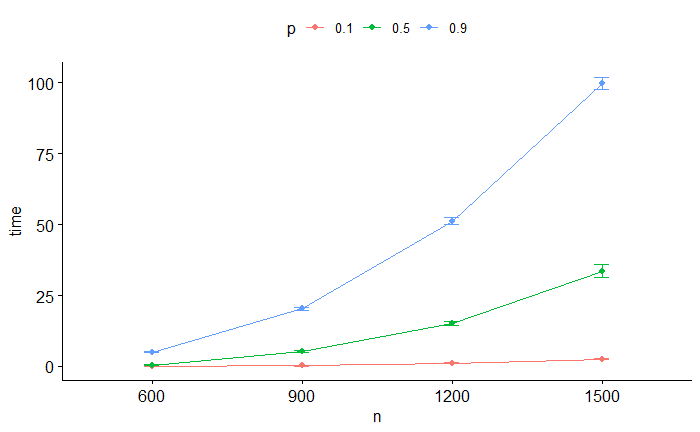
\includegraphics[width=1\textwidth]{ek_intplot2.png}
        \caption{EK boxplot para $p$}
        \label{fig:intplot-ek-p}
    \end{minipage}
\end{figure}

\subsection{Teste Two-Way ANOVA}

Em seguida é mostrada a tabela \ref{fig:anova-ek} obtida utilizando a função \emph{aov} do R para analisar os resultados obtidos e tomar uma decisão de rejeitar ou não rejeitar as hipóteses.

\begin{figure}[h]
    \centering
    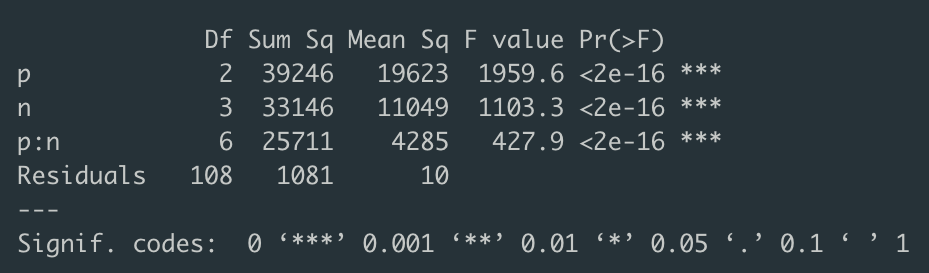
\includegraphics[width=0.7\linewidth]{ek-anova.png}
    \caption{Tabela ANOVA EK}
    \label{fig:anova-ek}
\end{figure}

\subsection{Validação pressupostos ANOVA}

Semelhante aos casos anteriores, na figura \ref{fig:pressupostos-mpm} podemos observar que tanto para o teste de Levene como para o teste de Shapiro-Wilk rejeitamos ambas as hipóteses nulas dos testes. 

\begin{figure}[h]
    \centering
    \begin{minipage}{0.45\textwidth}
        \centering
        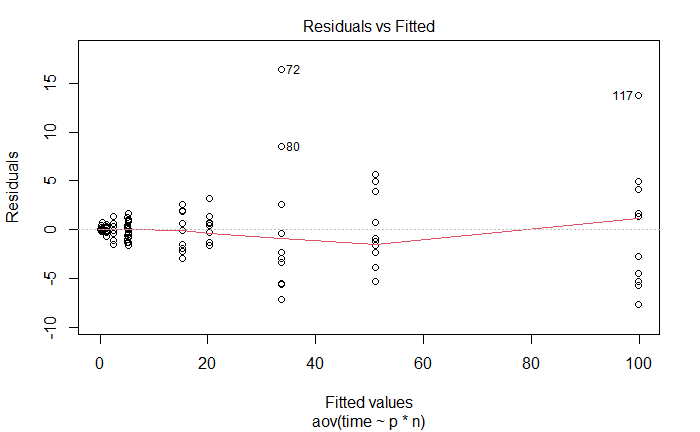
\includegraphics[width=1\textwidth]{res_plot_ek.png}
        \caption{EK Residuals vs Fitted plot}
        \label{fig:resplot-ek}
    \end{minipage}
    \hfill
    \begin{minipage}{0.45\textwidth}
        \centering
        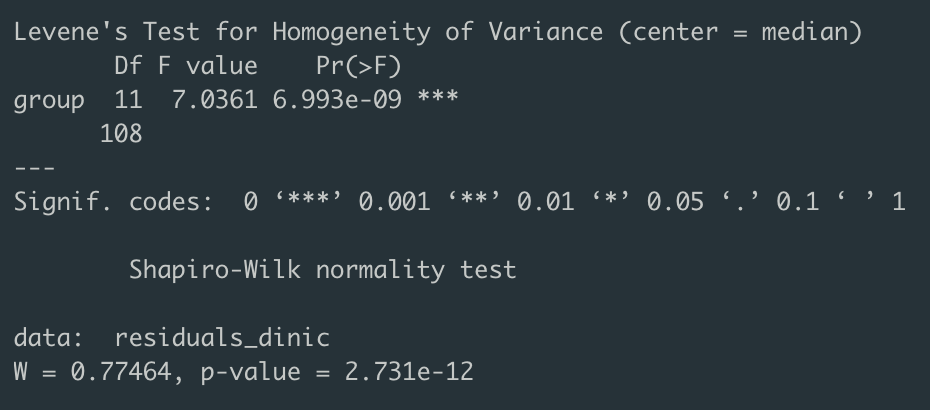
\includegraphics[width=1\textwidth]{pressupostos_ek.png}
        \caption{Pressupostos ANOVA}
        \label{fig:prssupostos-ek}
    \end{minipage}
\end{figure}

\subsection{Alternativa não paramétrica para Two-Way ANOVA}

Após verificar os pressupostos ANOVA, foi possível concluir que os pressupostos de normalidade e a homogeneidade das variações não foram validados. Dado isto foi utilizada a alternativa não paramétrica e os resultados podem ser observados na figura \ref{fig:randtest-ek}

\begin{figure}[h]
    \centering
    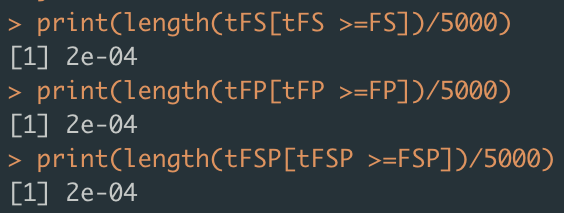
\includegraphics[width=0.5\linewidth]{rand_test_ek.png}
    \caption{Randomization test EK}
    \label{fig:randtest-ek}
\end{figure}

\section{Conclusões}

Como é possível ver na tabela ANOVA dos diferentes algoritmos, podemos ver que o p-value ($Pr(>F)$) é muito baixo, inferior ao nível de significância de 5\% para os fatores $n$ e $p$, sendo que temos evidências suficientes para rejeitar as hipóteses nulas $H_0^1$ $H_0^2$ $H_0^3$, ou seja, podemos concluir que existe um efeito significativo da variável categórica sobre a variável de resposta, neste caso a probabilidade sobre tempo.

Os pressupostos do teste ANOVA falharam para todos os algoritmos. Foi realizado o Levene test para os 3 algoritmos onde obtivemos evidências suficientes para rejeitar a hipótese nula $H_0$, ou seja, como o p-value é inferior a 0.05, sugere que as variâncias não são iguais em todas as combinações das duas variáveis categóricas, e que o pressuposto da homogeneidade das variâncias foi violado.
Também foi realizado o Shapiro-wilk test para os diferentes algoritmos, na qual obtivemos evidências para rejeitar a hipótese nula $H_0$, ou seja, como o p-value é inferior a 0.05, os resíduos não seguem uma distribuição normal.

Sendo que os pressupostos ANOVA não se verificaram, foi utilizada a alternativa não paramétrica para o Two-way ANOVA (randomization test), onde foi possível observar que os valores de p-value são inferiores ao nível de significância de 5\%, sendo que podemos rejeitamos a hipótese nula e concluímos que existe uma diferença significativa entre as médias do fator $p$ (probabilidade) para os diferentes níveis (0.1,0.5,0.9). 

Concluímos assim que, para os 3 algoritmos, tanto $n$ como $p$ têm um impacto significativo no tempo de execução e que existem interações significavas entre as duas variáveis. Assim somos levados a considerar falsa a hipótese $A$ formulada na secção \ref{sec:formulacao-hipoteses}, e verdadeiras as hipóteses $B$ e $C$.

\begin{thebibliography}{ht}
\bibitem{texbook}
\emph{R documentation}, \url{https://www.rdocumentation.org/}.

\bibitem{mei-course-materials}
Luís Paquete (2022), Materiais disponibilizados no âmbito da disciplina de MEI

\bibitem{Two way ANOVA}
Various authors, \emph{Statology: Two way ANOVA}, \url{https://www.statology.org/two-way-anova/}

\bibitem{Teste não paramétrico}
Various authors, \emph{Measuringu: Randomization Test}, \url{https://measuringu.com/randomization-test/}

\end{thebibliography}

\end{document}

